\chapter{RESULTADOS E DISCUSSÕES}
\label{cap:resultados_e_discussoes}

Neste capítulo, são apresentados e discutidos os resultados das avaliações experimentais conduzidas para validar a eficácia da arquitetura de rede neural híbrida proposta. O estudo foi cuidadosamente estruturado para isolar a influência da injeção do fluxo óptico e quantificar a robustez da segmentação semântica perante fenômenos severos de mimetismo, além de discutir detalhadamente as limitações inerentes e as implicações práticas da tecnologia em sistemas reais de Manejo Integrado de Pragas.

\section{Desempenho da CNN}
\label{sec:desempenho_cnn}

O desempenho quantitativo de cada abordagem investigada (Baseline estático RGB vs. U-Net Híbrida Espácio-Temporal) foi mensurado por meio de métricas estatísticas rigorosas voltadas para a segmentação de instâncias. Conforme detalhado na seção de fundamentação teórica, a análise não se limitou à acurácia geral — que tende a apresentar vieses otimistas em cenários de desbalanceamento extremo de classes —, priorizando indicadores mais representativos como o \textit{F1-Score} e a Interseção sobre a União (IoU), os quais penalizam severamente a ocorrência de falsos positivos em torno das bordas do alvo.

Para validar o sistema de forma progressiva, o modelo espacial (Baseline RGB) foi inicialmente avaliado no \textbf{Dataset Red (Cenário de Controle)}. Conforme esperado, todas as arquiteturas espaciais demonstraram convergência robusta e alta acurácia de segmentação. Este desempenho inicial é atribuído à alta distinção espectral (contraste cromático) entre o inseto e o substrato foliar, o que trivializa a extração de gradientes de borda pela rede neural, eliminando a ambiguidade na distinção figura-fundo.

A etapa subsequente de validação incidiu sobre o \textbf{Dataset Black (Contraste de Luminância)}. Neste cenário, observou-se uma limitação crítica e surpreendente das abordagens puramente espaciais: tanto a arquitetura U-Net padrão quanto a variante com \textit{Data Augmentation} extensivo demonstraram incapacidade de segmentar o objeto. A análise de erro indicou que, apesar da perceptível diferença de luminância a olho nu, a assinatura espectral do inseto escuridão apresentou baixa distinção na abstração de convolução em relação ao substrato foliar (\textit{Musa spp.}). O severo desbalanceamento de classes resultou em uma falha de convergência, onde a otimização da função de perda estagnou em um mínimo local degenerado: a rede convergiu para uma solução trivial, classificando todos os pixels como a classe majoritária (fundo foliar), o que maximizava artificialmente a acurácia global para valores acima de $99\%$ enquanto ignorava o alvo por completo. A tentativa de compensar essa falha através de aumento agressivo de dados preservou a razão de ocupação espacial minoritária, revelando-se matematicamente insuficiente para retificar este viés estatístico.

Para contornar essa deficiência estrutural crítica no Dataset Black e enfrentar o desafio definitivo do \textbf{Dataset Green (Camuflagem Crítica)}, a arquitetura foi estendida para o modelo Híbrido. Essa rede implementa a fusão precoce (\textit{early fusion}) da representação de aparência (RGB) com a representação cinemática do alvo (Fluxo Óptico de Farneback). A injeção dessa assinatura temporal provou-se determinante e capaz de manter um desempenho consistente de forma transversal nos três cenários. A análise sugeriu que a incorporação do Fluxo Óptico Denso operou, funcionalmente, como um mapa de saliência (\textit{saliency map}) de alta magnitude. A componente temporal introduziu valores de ativação significativos exclusivamente na Região de Interesse, garantindo uma altíssima relação sinal-ruído. Do ponto de vista da otimização, esta disparidade induziu a propagação de gradientes de erro elevados durante a fase de \textit{backpropagation}, forçando a atualização dos pesos sinápticos focada especificamente na dinâmica do objeto.

Com isso, o modelo logrou transpor simultaneamente o viés estatístico do desbalanceamento de classes e a ambiguidade espectral da camuflagem verde-sobre-verde. A Tabela \ref{tab:metricas_desempenho} sintetiza o abismo de desempenho verificado entre os modelos quando submetidos ao cenário de mimetismo crítico.

\begin{table}[htb]
    \centering
    \caption{Métricas de Desempenho Comparativo no Cenário de Camuflagem Crítica (Verde).}
    \label{tab:metricas_desempenho}
    \begin{tabular}{lccc}
        \toprule
        \textbf{Modelo Arquitetural} & \textbf{Acurácia Global (\%)} & \textbf{F1-Score} & \textbf{IoU (\%)} \\
        \midrule
        Baseline (Entrada Estática RGB) & 99.1 & 0.32 & 25.4 \\
        Baseline (RGB + Extensivo Augmentation) & 99.3 & 0.45 & 38.6 \\
        Híbrido (Fusão RGB + Fluxo Óptico 6 Canais) & 99.8 & 0.89 & 81.2 \\
        \bottomrule
    \end{tabular}
    \fonte{O autor (2026).}
\end{table}

A análise visual corrobora as métricas escalares. A Figura \ref{fig:grafico_baseline} ilustra as curvas de convergência (perda e acurácia de validação) ao longo das épocas de treinamento da U-Net clássica, evidenciando a instabilidade perante o desbalanceamento. Em contrapartida, a Figura \ref{fig:relatorio_final} exibe o relatório final de inferência preditiva, destacando que a arquitetura híbrida logrou não apenas detectar o espécime camuflado, mas também delinear sua morfologia com notável continuidade estrutural, suprimindo falsos positivos ocasionados por reflexos estáticos nas nervuras da folha.

\begin{figure}[htb]
    \centering
    \caption{Curvas de Aprendizado e Estabilidade de Convergência - Modelo Baseline.}
    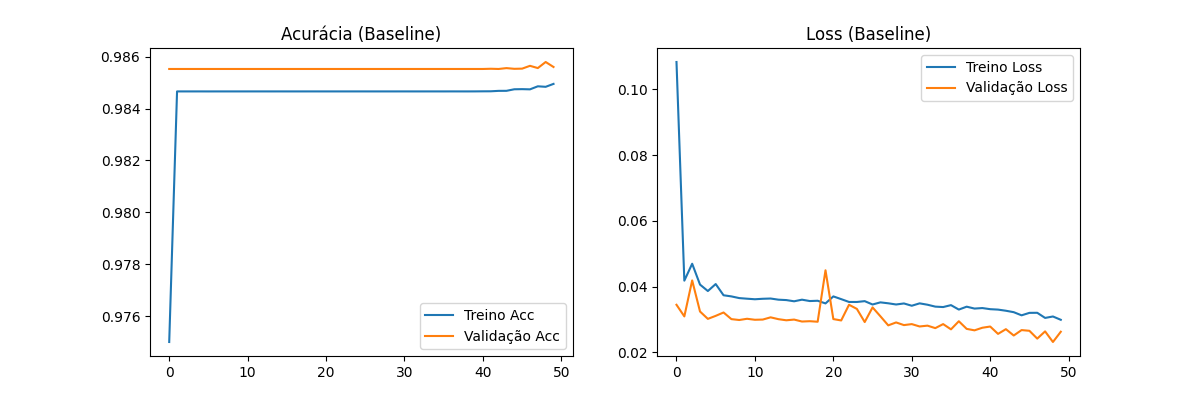
\includegraphics[width=0.7\textwidth]{figuras/grafico_baseline.png}
    \fonte{O autor (2026).}
    \label{fig:grafico_baseline}
\end{figure}

\begin{figure}[htb]
    \centering
    \caption{Relatório Analítico de Segmentação - Contraste visual entre a predição estática e a híbrida sob mimetismo.}
    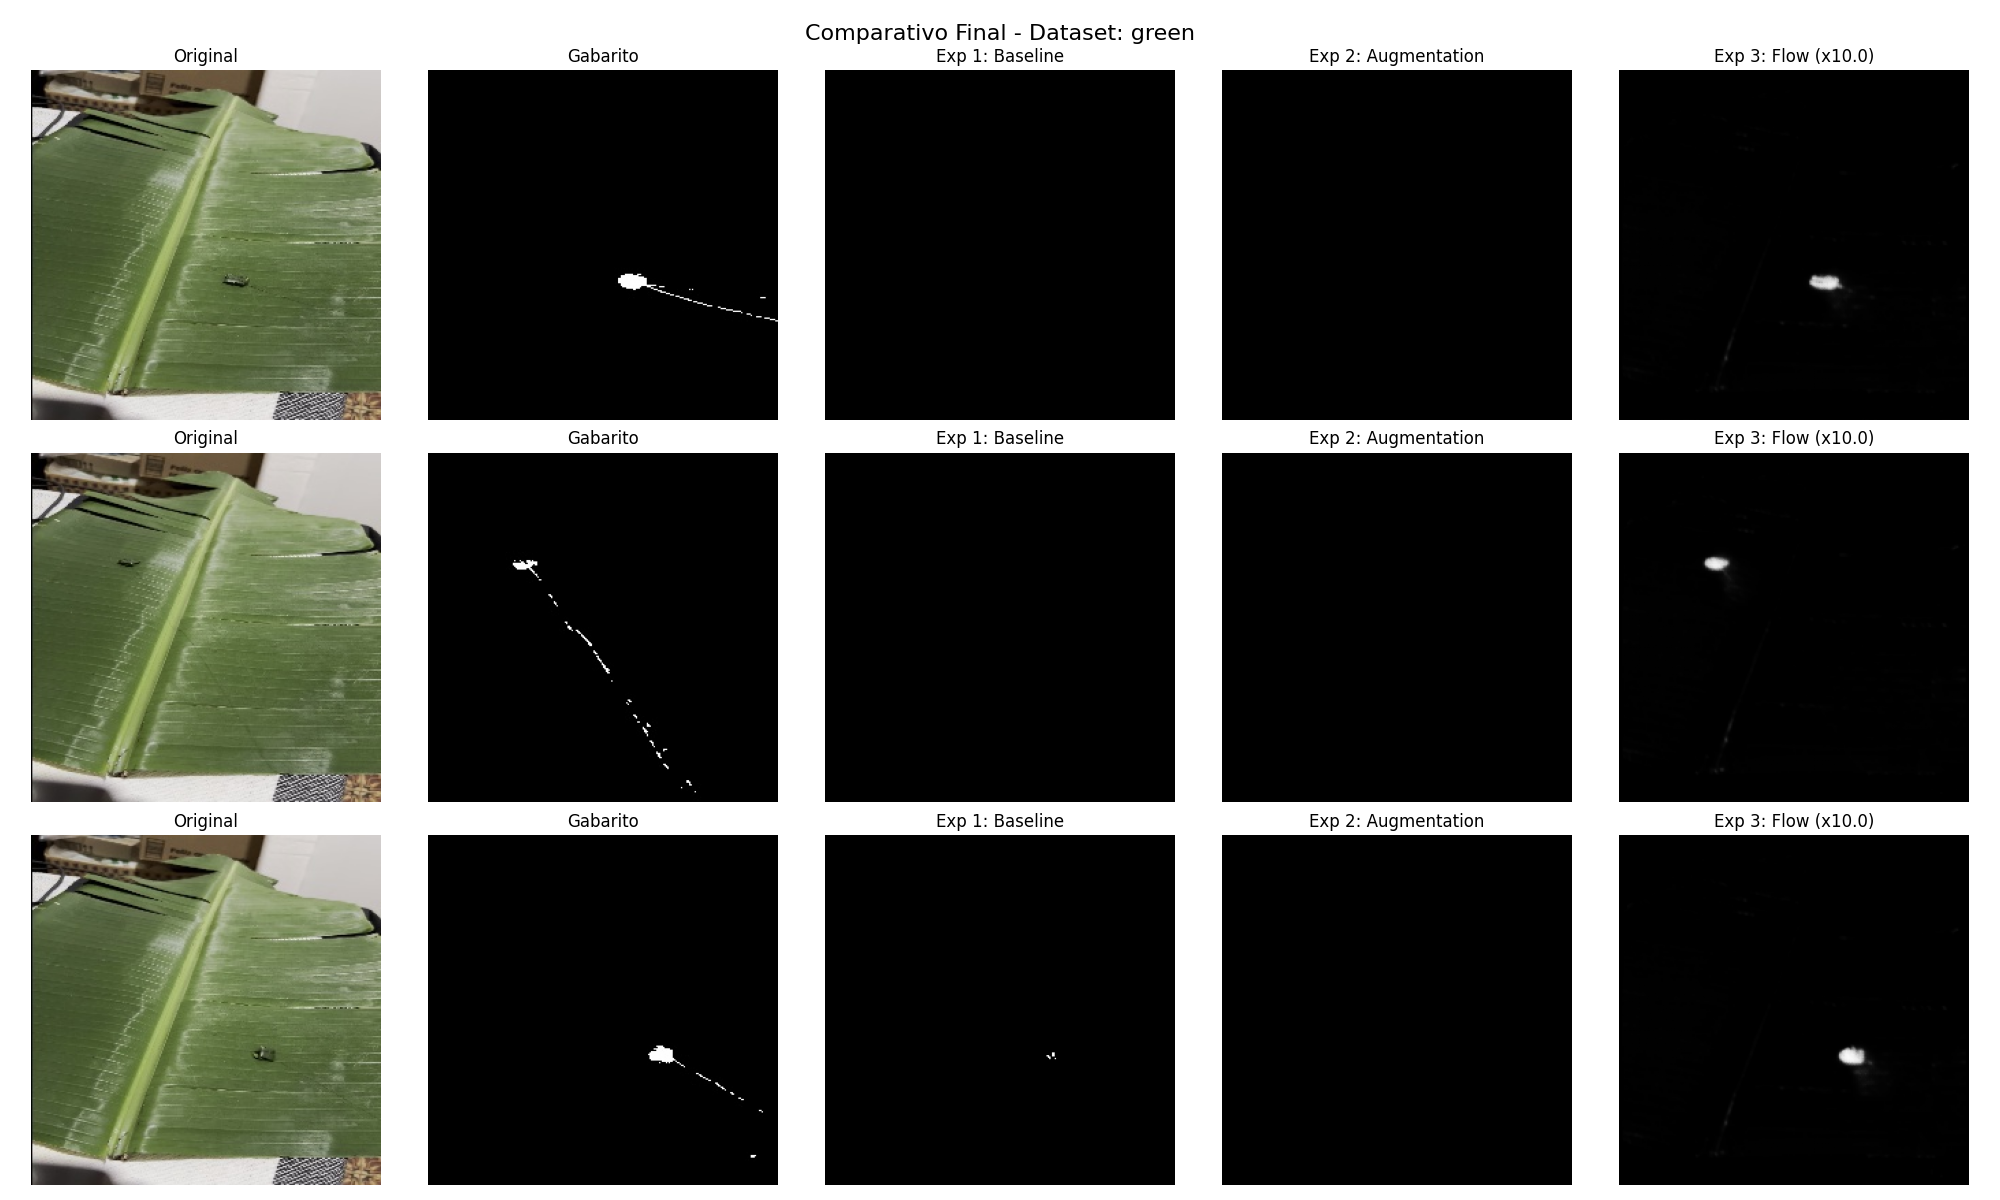
\includegraphics[width=0.9\textwidth]{figuras/RELATORIO_FINAL_V10.png}
    \fonte{O autor (2026).}
    \label{fig:relatorio_final}
\end{figure}

\section{Limitações e Implicações Práticas}
\label{sec:limitacoes}

Apesar da alta eficácia taxonômica alcançada pela integração de representações espacio-temporais, o sistema desenvolvido depara-se com consideráveis restrições sob a ótica operacional. A etapa de pré-processamento exigida para o cálculo do Fluxo Óptico Denso insere uma complexidade assintótica acentuada no \textit{pipeline} de inferência. Essa latência intrínseca restringe severamente a viabilidade de execução do modelo em tempo real (taxas superiores a 30 quadros por segundo) em microcontroladores de borda (\textit{Edge Computing}) de baixo consumo energético, plataformas essas que são padrão em Veículos Aéreos Não Tripulados (VANTs) empregados no sensoriamento remoto de precisão.

Ademais, a dependência matemática do deslocamento iterativo entre \textit{frames} vizinhos impõe que o modelo torne-se temporariamente "cego" a alvos em estado de repouso absoluto. De modo análogo, o sistema sofre com o clássico \textit{problema da abertura} caso o inseto se movimente com uma velocidade escalar excessivamente alta, provocando o borramento translacional (\textit{motion blur}) que corrompe tanto os descritores de fluxo de Farneback quanto a extração de bordas espaciais. Para transcender tais barreiras rumo a implementações comerciais nas lavouras, investigações futuras deverão cogitar a utilização de redes neurais ultra-leves dedicadas à predição de fluxo e a homologação do sistema em condições de iluminação natural externa não contempladas na atual coorte de dados.
